\documentclass[10pt]{article}
\usepackage[a3paper,landscape,margin=1cm]{geometry}
\usepackage[utf8]{inputenc}
\usepackage[T1]{fontenc}
\usepackage{lmodern}
\usepackage{xcolor}
\usepackage{tikz}
\usepackage{tcolorbox}
\usepackage{amsmath}
\usepackage{amssymb}
\usepackage[default]{lato}
\tcbuselibrary{skins,breakable}

% --- Paleta dark (consistente con plots) ---
\definecolor{bg}{HTML}{0d1117}
\definecolor{card}{HTML}{161b22}
\definecolor{border}{HTML}{30363d}
\definecolor{text}{HTML}{e6edf3}
\definecolor{label}{HTML}{8b949e}
\definecolor{title}{HTML}{f9e64f}
\definecolor{tp}{HTML}{58a6ff}
\definecolor{gen}{HTML}{3fb950}
\definecolor{formula}{HTML}{d2a8ff}

\pagecolor{bg}
\color{text}
\pagestyle{empty}
\setlength{\parindent}{0pt}

% --- Estilo de tarjeta ---
\newtcolorbox{card}[2]{
  colback=card, colframe=#1, coltitle=text,
  arc=3pt, boxrule=0.9pt, left=8pt, right=8pt, top=5pt, bottom=5pt,
  title=\textbf{\large #2}, fonttitle=\color{text},
  attach boxed title to top left={xshift=10pt, yshift=-8pt},
  boxed title style={colback=#1, sharp corners, boxrule=0pt, top=2pt, bottom=2pt, left=6pt, right=6pt},
  enhanced,
}

\newcommand{\fb}[1]{{\color{label}\small #1}}
\newcommand{\tip}[2]{{\color{#1}\textbf{$\blacktriangleright$\ #2}}}
\newcommand{\formulabox}[1]{{\color{formula}\large $\displaystyle #1$}}

\begin{document}

% ========== HEADER ==========
\begin{center}
{\Huge\textbf{MÉTRICAS DEL EJ2}}\\[2pt]
{\color{label}\itshape SIA TP3 · ITBA · Clasificación multiclase de dígitos (10 clases, 1 minoritaria)}
\end{center}
\vspace{4pt}

% ========== SECCIÓN 1 ==========
{\color{tp}\textbf{\large 1. LO QUE USAMOS PARA DECIDIR EN EL TP}}\\
\fb{Dos métricas en toda cell. val\_acc rankea, val\_loss desempata y monitorea overfitting.}
\vspace{6pt}

\noindent
\begin{minipage}[t]{0.49\textwidth}
\begin{card}{tp}{\texttt{val\_acc} — Validation Accuracy}
\formulabox{\mathrm{val\_acc} = \frac{1}{N_{val}} \sum_i \mathbf{1}[\hat{y}_i = y_i]}\\[6pt]
\fb{Fracción de imágenes del fold val que el modelo clasifica bien.}\\[3pt]
\fb{\textbf{Cálculo:} forward → softmax → argmax → match. Media sobre k-folds × seeds.}\\[3pt]
\tip{tp}{Métrica PRINCIPAL de ranking.}
\end{card}
\end{minipage}\hfill
\begin{minipage}[t]{0.49\textwidth}
\begin{card}{tp}{\texttt{val\_loss} — Cross-Entropy en validación}
\formulabox{\mathrm{CE} = -\frac{1}{N} \sum_i \sum_c y_{i,c}\,\log \hat{p}_{i,c}}\\[6pt]
\fb{La loss que el modelo MINIMIZA al entrenar. Mide calibración de probabilidades.}\\[3pt]
\fb{\textbf{Cálculo:} log de la prob softmax de la clase real, promediado.}\\[3pt]
\tip{tp}{TIE-BREAKER cuando val\_acc empata. Menor CE = menos overfit.}
\end{card}
\end{minipage}
\vspace{14pt}

% ========== SECCIÓN 2 ==========
{\color{gen}\textbf{\large 2. MÉTRICAS DE CLASIFICACIÓN — REFERENCIA GENERAL}}\\
\fb{Las 4 fundamentales + variantes multiclase. Ancla teórica para defensa oral.}
\vspace{6pt}

% Grid 3×2 de tarjetas pequeñas
\noindent
\begin{minipage}[t]{0.325\textwidth}
\begin{card}{gen}{Accuracy}
\formulabox{\mathrm{acc} = \frac{TP + TN}{TP + FP + TN + FN}}\\[6pt]
\fb{Aciertos sobre total. Engaña con desbalance.}\\[3pt]
\tip{gen}{Útil con clases balanceadas.}
\end{card}
\end{minipage}\hfill
\begin{minipage}[t]{0.325\textwidth}
\begin{card}{gen}{Precision (clase $c$)}
\formulabox{P_c = \frac{TP_c}{TP_c + FP_c}}\\[6pt]
\fb{De lo que predije como $c$, ¿cuánto era $c$?}\\[3pt]
\tip{gen}{Importa si FPs son caros (spam, fraude).}
\end{card}
\end{minipage}\hfill
\begin{minipage}[t]{0.325\textwidth}
\begin{card}{gen}{Recall (clase $c$)}
\formulabox{R_c = \frac{TP_c}{TP_c + FN_c}}\\[6pt]
\fb{De los $c$ reales, ¿cuántos detecté?}\\[3pt]
\tip{gen}{Importa si FNs son caros (cáncer).}
\end{card}
\end{minipage}
\vspace{6pt}

\noindent
\begin{minipage}[t]{0.325\textwidth}
\begin{card}{gen}{F1-score (clase $c$)}
\formulabox{F1_c = \frac{2\,P_c\,R_c}{P_c + R_c}}\\[6pt]
\fb{Media armónica de $P$ y $R$.}\\[3pt]
\tip{gen}{Castiga si $P$ o $R$ es bajo.}
\end{card}
\end{minipage}\hfill
\begin{minipage}[t]{0.325\textwidth}
\begin{card}{gen}{Macro F1}
\formulabox{\mathrm{macroF1} = \frac{1}{C} \sum_c F1_c}\\[6pt]
\fb{Promedio sin pesar por frecuencia.}\\[3pt]
\tip{gen}{Default con desbalance. ESTE TP.}
\end{card}
\end{minipage}\hfill
\begin{minipage}[t]{0.325\textwidth}
\begin{card}{gen}{Weighted / Micro F1}
\formulabox{\mathrm{wF1} = \sum_c \tfrac{n_c}{N} F1_c}\\[6pt]
\fb{Weighted: pesa por frecuencia. Micro: pool global ($\equiv$ acc).}\\[3pt]
\tip{gen}{Weighted ESCONDE clases raras.}
\end{card}
\end{minipage}
\vspace{12pt}

% ========== FOOTER: matriz + regla ==========
\noindent
\begin{minipage}[t]{0.62\textwidth}
\begin{tcolorbox}[colback=card, colframe=border, arc=3pt, boxrule=0.9pt,
                  left=8pt, right=8pt, top=4pt, bottom=4pt]
{\textbf{\color{text}Matriz de confusión por clase $c$}}\hfill\fb{TP/FP/FN/TN se cuentan por clase, después se agregan.}\\[4pt]
\centering
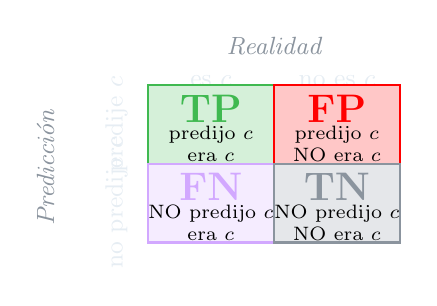
\begin{tikzpicture}[every node/.style={font=\small\color{text}, align=center}]
  % Headers
  \node at (1.6,2.55) {\color{label}\itshape Realidad};
  \node at (0.8,2.1) {es $c$}; \node at (2.4,2.1) {no es $c$};
  \node[rotate=90] at (-1.3,1.0) {\color{label}\itshape Predicción};
  \node[rotate=90] at (-0.4,1.55) {predije $c$};
  \node[rotate=90] at (-0.4,0.55) {no predije $c$};
  % Cells
  \fill[gen!22, draw=gen, line width=0.8pt] (0.0,1.05) rectangle (1.6,2.05);
  \node[color=gen,font=\Large\bfseries] at (0.8,1.75) {TP};
  \node[font=\scriptsize] at (0.8,1.30) {predijo $c$\\era $c$};

  \fill[red!22, draw=red, line width=0.8pt] (1.6,1.05) rectangle (3.2,2.05);
  \node[color=red,font=\Large\bfseries] at (2.4,1.75) {FP};
  \node[font=\scriptsize] at (2.4,1.30) {predijo $c$\\NO era $c$};

  \fill[formula!22, draw=formula, line width=0.8pt] (0.0,0.05) rectangle (1.6,1.05);
  \node[color=formula,font=\Large\bfseries] at (0.8,0.75) {FN};
  \node[font=\scriptsize] at (0.8,0.30) {NO predijo $c$\\era $c$};

  \fill[label!22, draw=label, line width=0.8pt] (1.6,0.05) rectangle (3.2,1.05);
  \node[color=label,font=\Large\bfseries] at (2.4,0.75) {TN};
  \node[font=\scriptsize] at (2.4,0.30) {NO predijo $c$\\NO era $c$};
\end{tikzpicture}
\end{tcolorbox}
\end{minipage}\hfill
\begin{minipage}[t]{0.36\textwidth}
\begin{tcolorbox}[colback=card, colframe=title, arc=3pt, boxrule=1.2pt,
                  left=8pt, right=8pt, top=4pt, bottom=4pt]
{\color{title}\textbf{Regla 4 del CLAUDE.md}}\\[4pt]
{\textbf{\color{text}Reportar SIEMPRE el set completo:}}\\[2pt]
\hspace{6pt}1.\ Loss de entrenamiento (CE en multiclase)\\
\hspace{6pt}2.\ Accuracy + Precision + Recall + F1\\
\hspace{6pt}3.\ Multiclase $\to$ {\color{title}\textbf{macro-average}}\\[6pt]
\fb{Las dos familias responden preguntas distintas:}\\[1pt]
\hspace{2pt}{\color{tp}\textbf{CE}} $\to$ qué tan calibrada está la prob.\\
\hspace{2pt}{\color{gen}\textbf{P/R/F1/Acc}} $\to$ qué tan bien clasifica argmax.
\end{tcolorbox}
\end{minipage}

\end{document}
